\begin{figure}\centering
	\subfloat[]{
		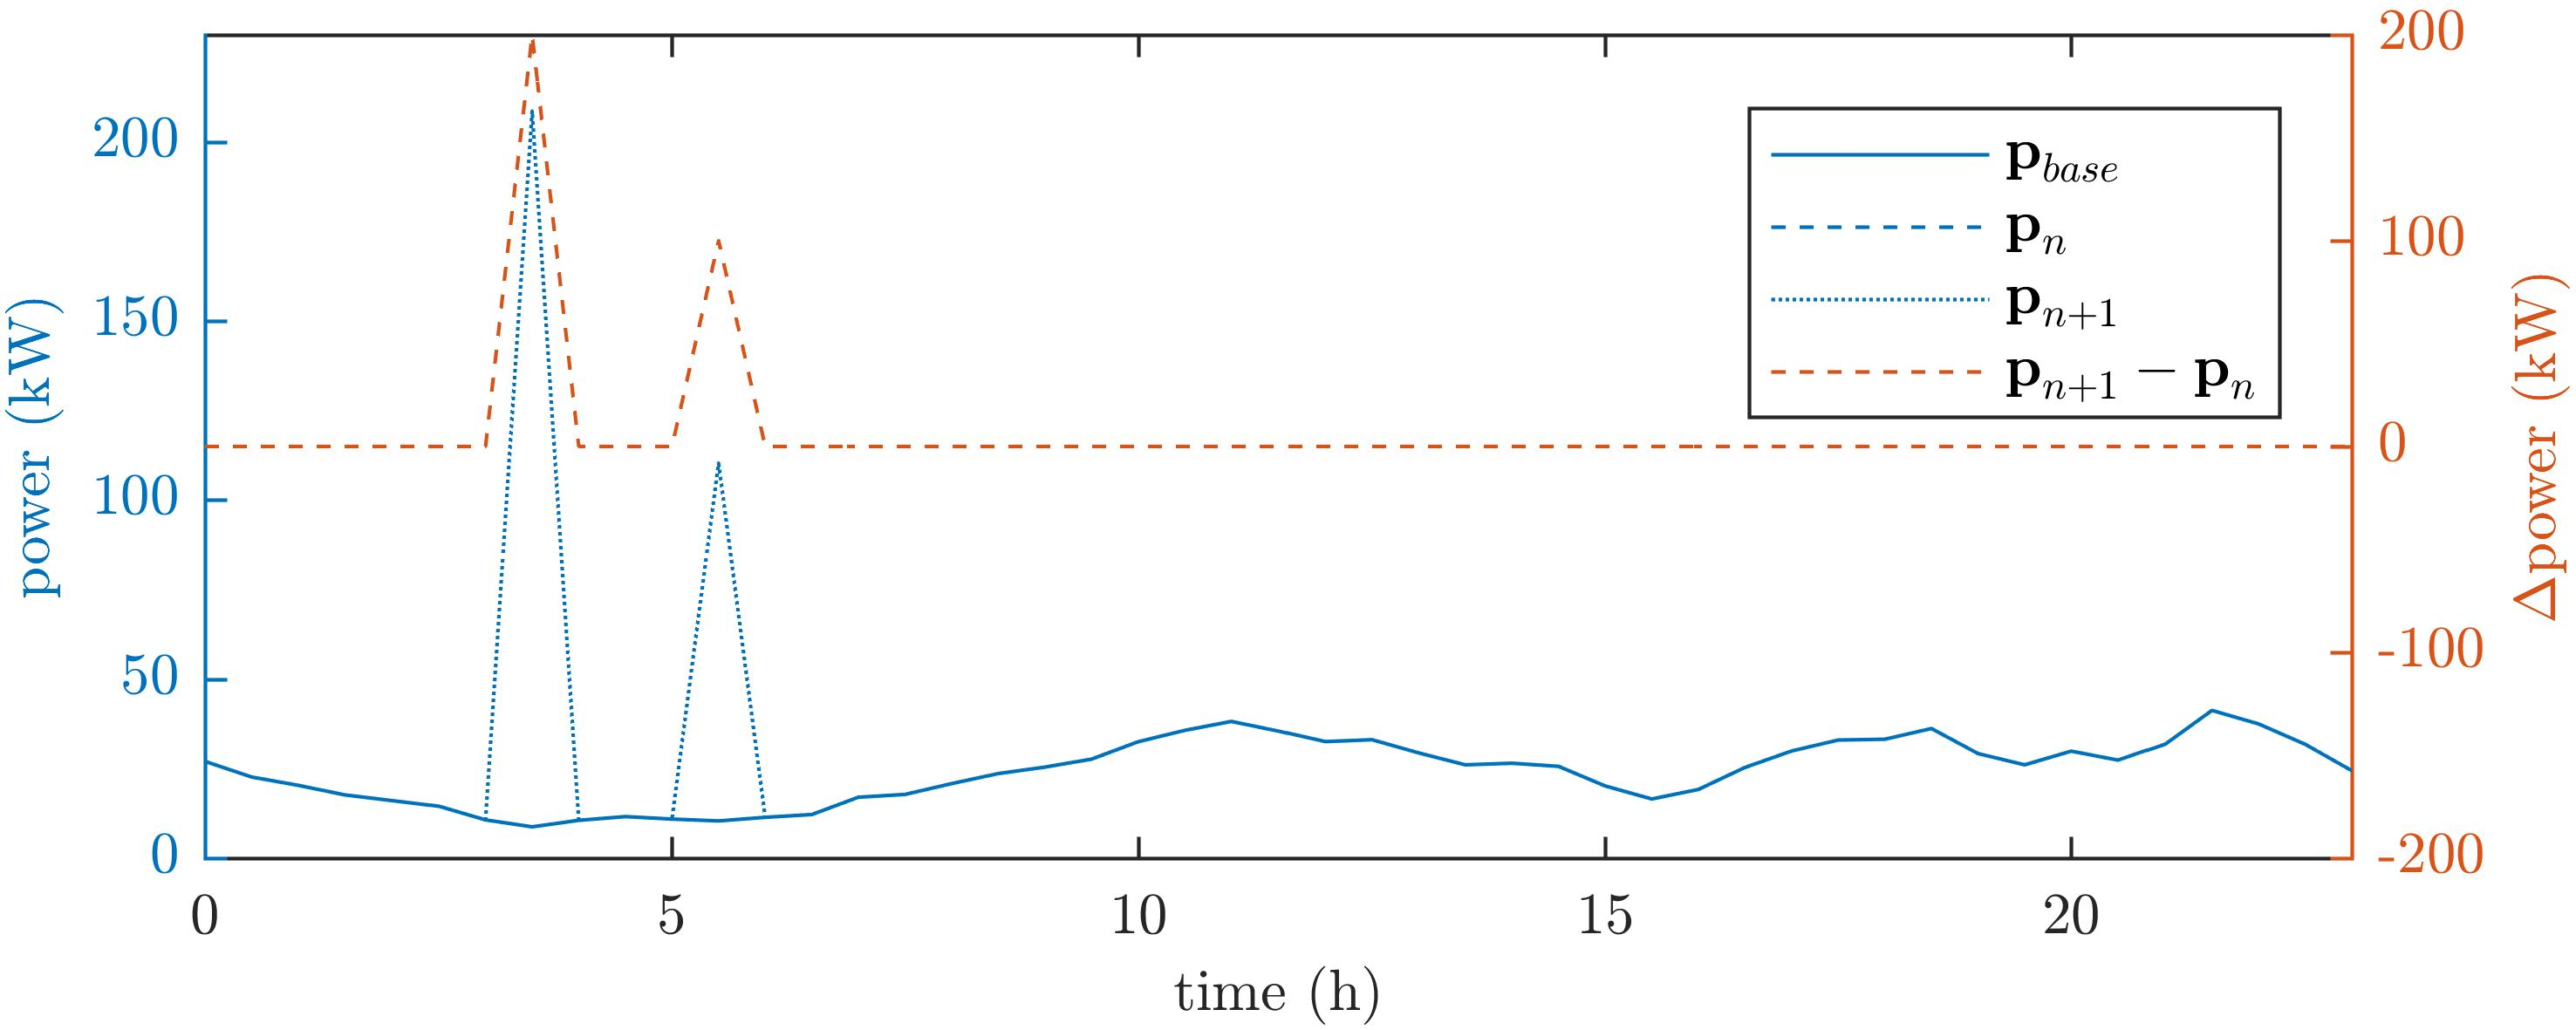
\includegraphics[height=4.5cm]{_chapter3/fig/oscillation/ts-i0001}
		\label{ch3:subfig:oscillation-1}
	}\\
	\subfloat[]{
		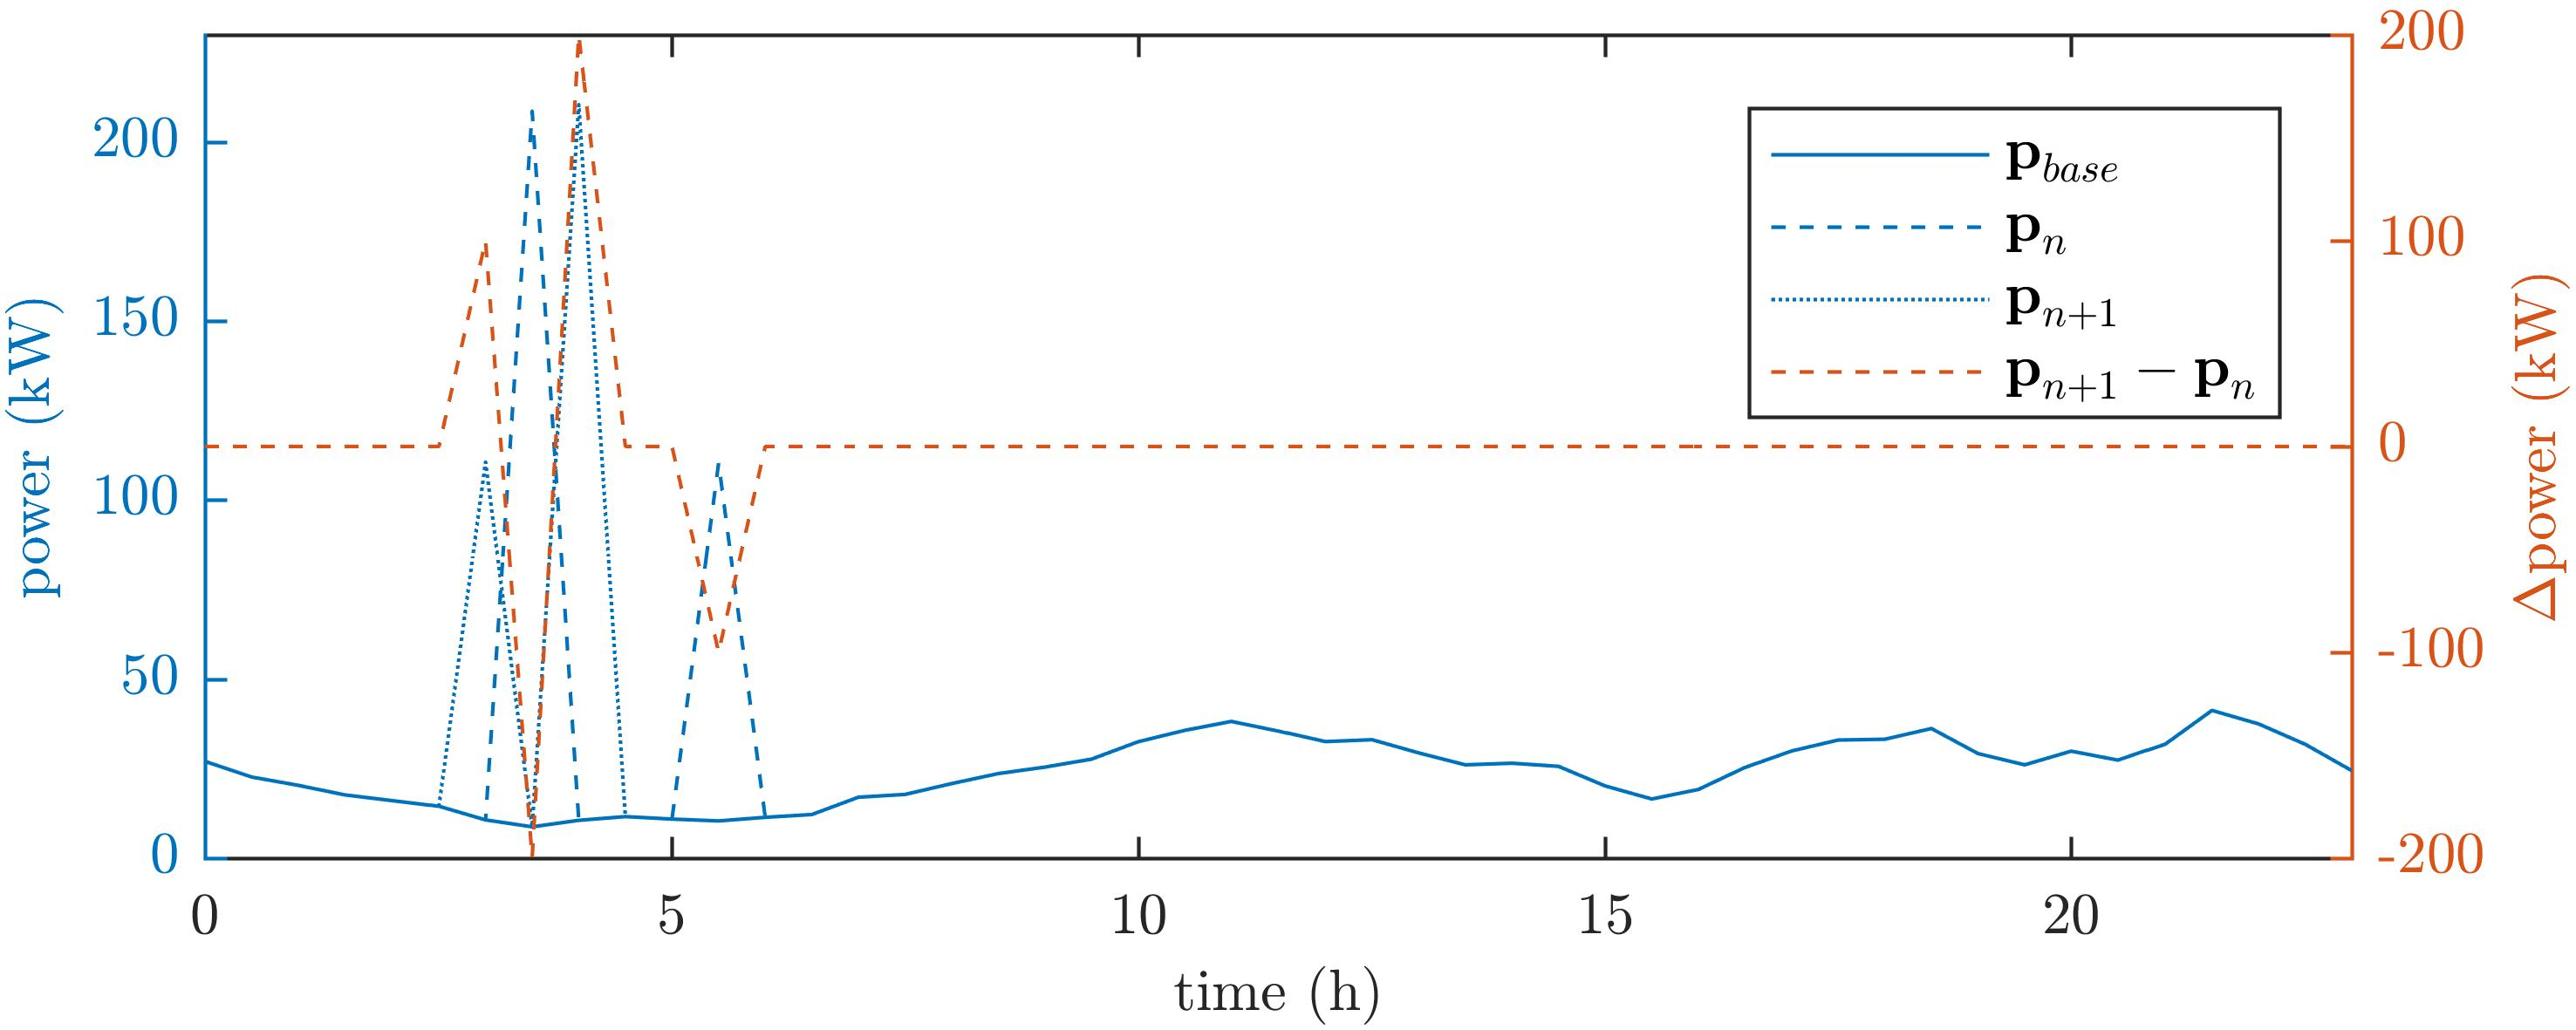
\includegraphics[height=4.5cm]{_chapter3/fig/oscillation/ts-i0002}
		\label{ch3:subfig:oscillation-2}
	}\\
	\subfloat[]{
		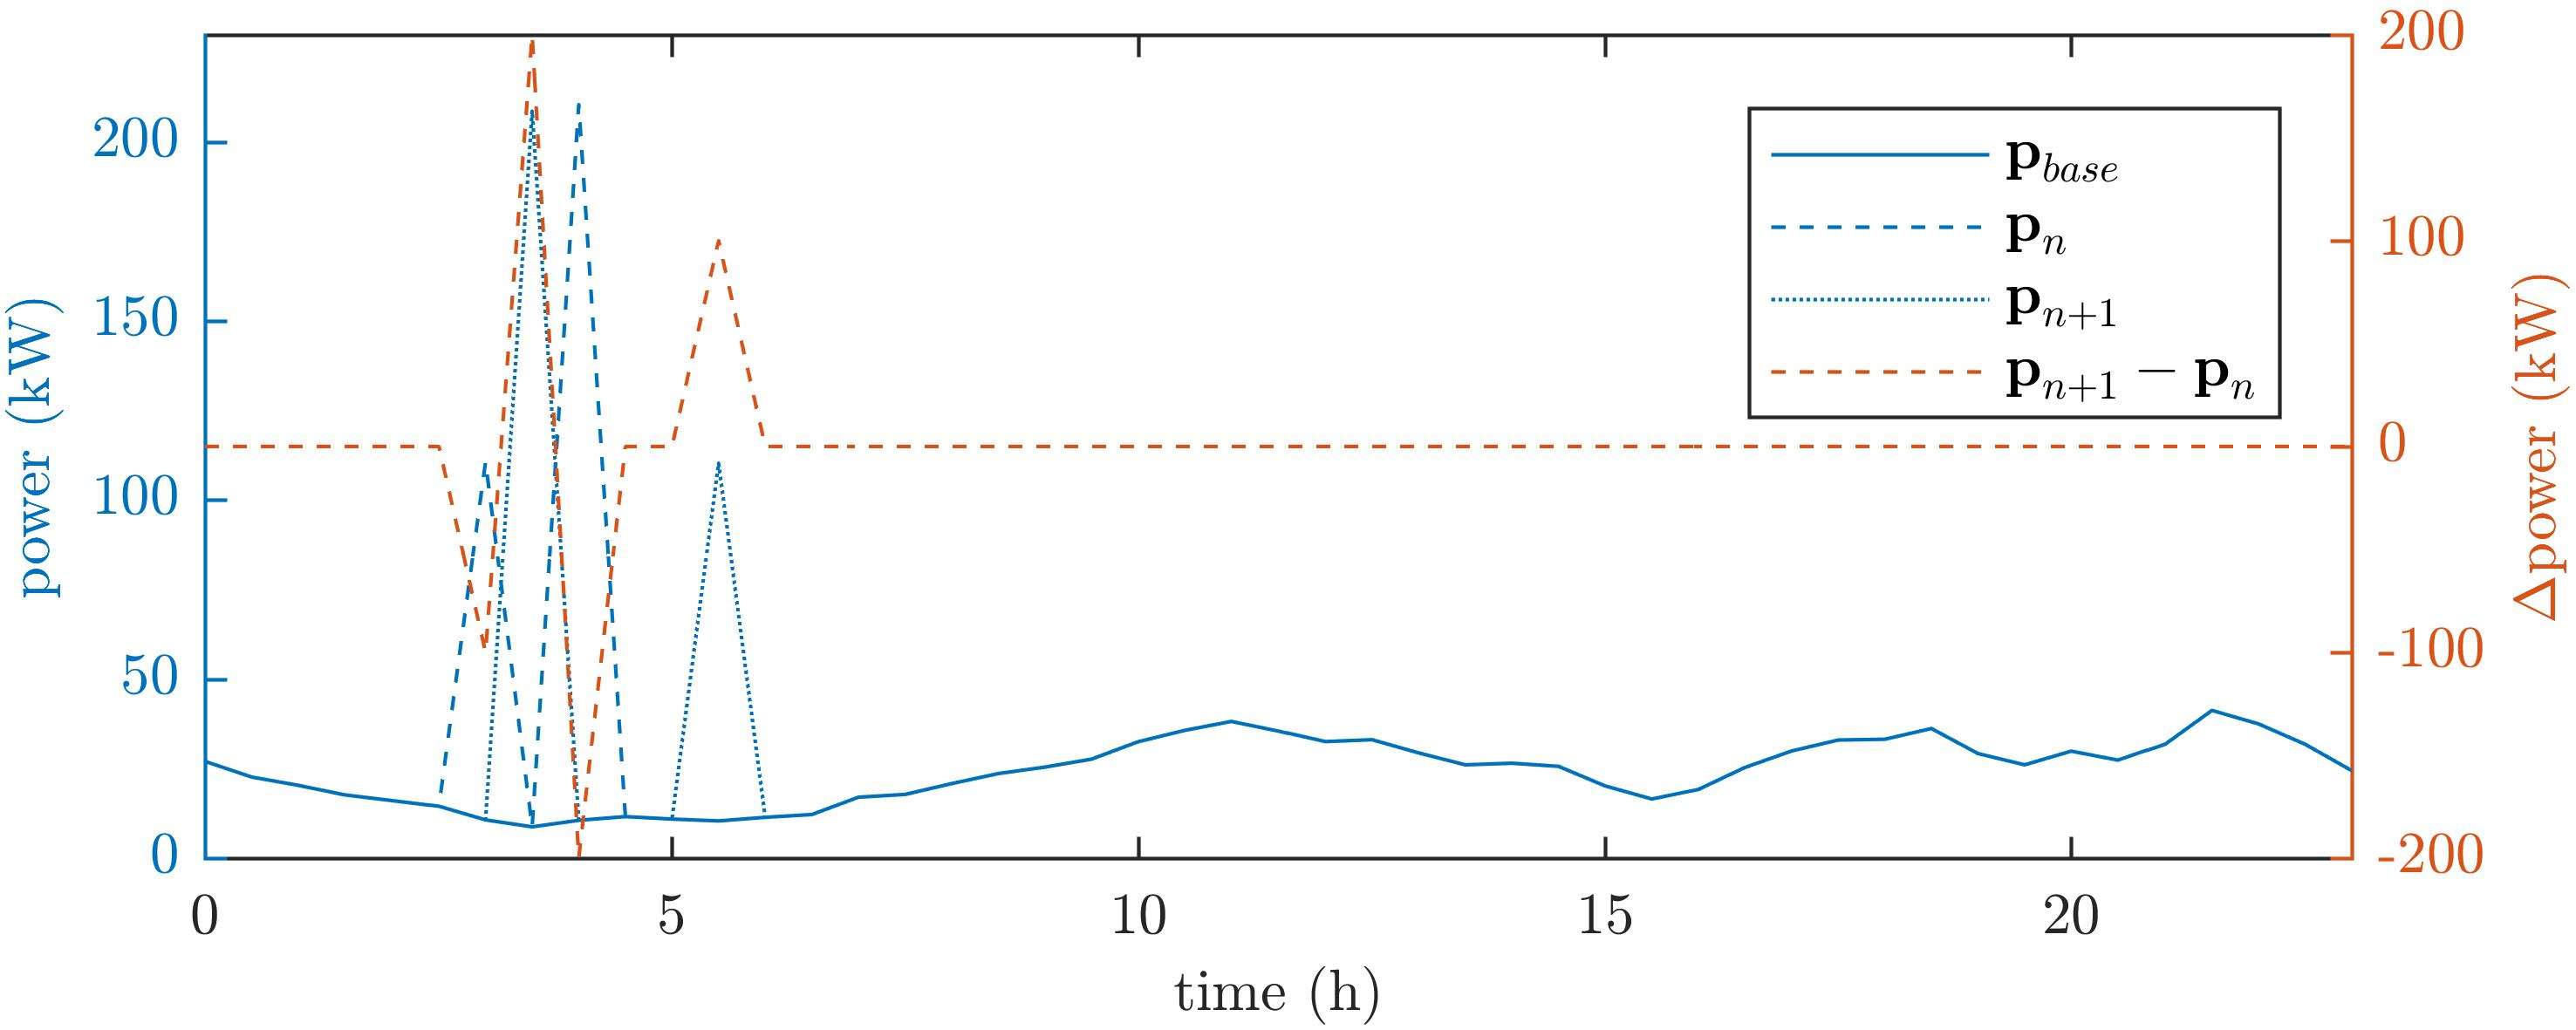
\includegraphics[height=4.5cm]{_chapter3/fig/oscillation/ts-i0003}
		\label{ch3:subfig:oscillation-3}
	}\\
	\subfloat[]{
		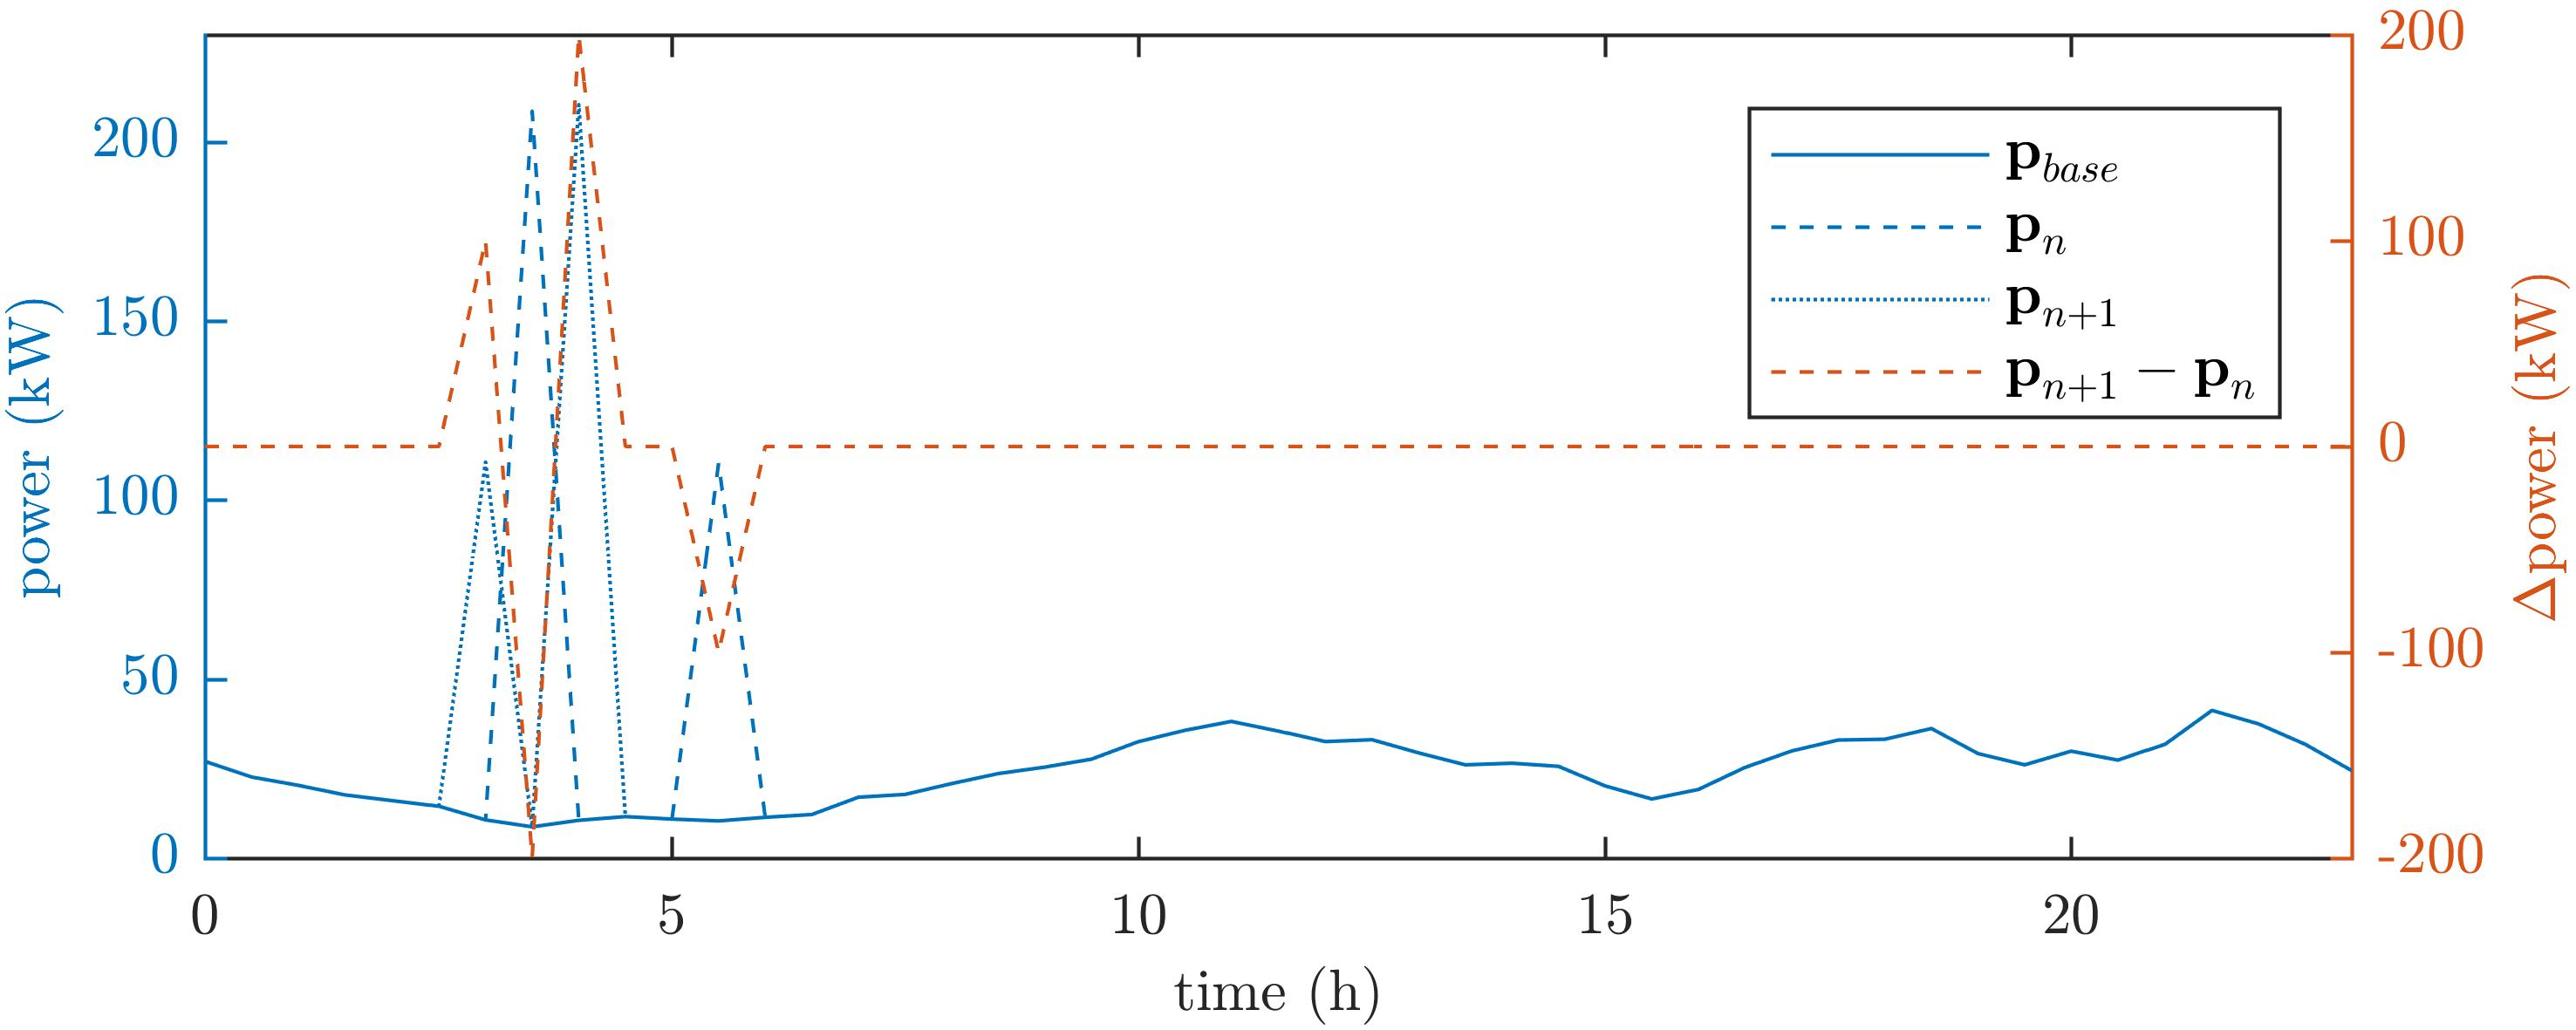
\includegraphics[height=4.5cm]{_chapter3/fig/oscillation/ts-i0100}
		\label{ch3:subfig:oscillation-last}
	}
\caption{Time series evolution for $\alpha=1.00$ and $\beta=1.00$, where (a) is at $n=1$, (b) is at $n=2$, (c) is at $n=3$, and (d) is at $n=N-1$.}
\label{ch3:fig:oscillation}
\end{figure}